\chapter{Analyse}
Die Analyse untersucht die bestehende Web Applikation und fasst die Anforderungen zusammen. Danach wird die Plattform und die passende Hardware dazu evaluiert und in Form einer Kaufempfehlung an die cnlab AG weitergeleitet. Es werden die verwendeten Technologien sowie ein kurzer Exkurs zu anderen Lösungen angesprochen.

\section{Requirements}
\label{sec:requirements}
Die Anforderungen an die \textit{RadioTour} Applikation ergeben sich aus den Features der bisherigen Web Applikation und den Verbesserungsvorschlägen des \textit{RadioTour} Speakers. Im Anhang \ref{ref:usecases} sind sämtliche UseCases der bisherigen Applikation aufgeführt. Im folgenden Abschnitt werden die Funktionen, welche in diesem Projekt implementiert sind, aufgeführt.

\subsection{Funktionale Anforderungen}
Die funktionalen Anforderungen sind in drei Prioritätsstufen eingeteilt:

\textbf{zwingende Anforderungen (must)}
\begin{itemize}
\item Fahrerliste, Etappen und Marschtabellen importieren
\item Fahrer ansehen, sortieren und bearbeiten
\item Gruppen bilden und Rückstand angeben
\item Gruppen auflösen
\item Events für Fahrer erfassen (Sturz, Arzt, Aufgabe)
\item Rennsituation an den Server übermitteln
\item Spezialklassemente und Wertungen erstellen und Fahrer zuweisen
\item Maillots erfassen und bearbeiten
\item Persistierung der Daten auf dem Gerät

\end{itemize}


\textbf{optionale Anforderungen (can)}
\begin{itemize}
\item Aktuelle Rennkilometer und Rennzeit anzeigen
\item Stoppuhr
\item Aktuelle Position durch GPS bestimmen
\item Events für Fahrer an den Server übermitteln
\end{itemize}


\textbf{wünschenswerte Anforderungen (nice to have)}
\begin{itemize}
\item Aktuelle Position des \textit{RadioTour Speakers} in der Marschtabelle anzeigen
\item \gls{splashscreen} beim Start der Applikation
\end{itemize}

\subsection{Nicht funktionale Anforderungen}
Im Umfeld eines Live Sport Events spielen neben den funktionalen Anforderungen an ein Software Produkt auch nicht funktionale Anforderungen eine wichtige Rolle. So muss z.B. das UserInterface Fehler bei der Eingabe tolerieren bzw. korrigierbar machen. Die Bedienung muss flüssig verlaufen und zu jedem Zeitpunkt muss der Status der Applikation sichtbar sein. Die für \textit{RadioTour} relevanten nicht funktionalen Anforderungen sind im Folgenden aufgelistet.

\begin{itemize}
\item Mobilfunkverbindung ist nicht immer gewährleistet, keine Daten dürfen dadurch verloren gehen
\item Informationen müssen auch bei direktem Sonnenlicht gut lesbar sein
\item Angenehme, flüssige und selbsterklärende Bedienung der Applikation
\end{itemize}

Weitere nicht funktionale Anforderungen beziehen sich auch auf die Hardware an sich und sind im Kapitel \ref{kap:kaufempfehlung} bereits aufgeführt.

\section{Evaluation und Kaufempfehlung}
\label{kap:kaufempfehlung}
Die Evaluation der Zielplattform war ein wichtiger Faktor für die weitere Entwicklung der Arbeit. Aus diesem Grund stand diese ganz zu Beginn der Arbeit an. Zur Auswahl standen die beiden marktführenden Betriebssysteme Android (Google) und iOS (Apple). Als Grundlage für die Evaluation dienten die folgenden Kriterien:
\begin{itemize}
\item Vorkenntnisse der Programmiersprachen Java bzw. Objective-C
\item Möglichkeiten zum UserInterface Design
\item Programmierumgebung, \gls{ide}
\item Mögliche Vertriebskanäle der Applikation
\item Nutzbarkeit von externen Geräten und Schnittstellen
\item Vielfalt von Informationsquellen im Internet
\end{itemize}
Die Kriterien werden in einer Nutzwertanalyse gewichtet und bewertet. Insbesondere die Vorkenntnisse in Java sind  ausschlaggebend für den Entscheid, die Applikation für die Androidplattform zu entwickeln. Dieser Entscheid ist in Absprache mit Herrn Heinzmann getroffen worden. Die gesamte Liste der Kriterien mit der jeweiligen Gewichtung sowie eine ausführliche Erläuterung befinden sich im Anhang \ref{ref:kriterien}.
\\

Für die Auswahl eines geeigneten Tablets wird im nächsten Schritt ein Kriterienkatalog definiert mit zwingenden und optionalen Kriterien für das Gerät. Die zwingenden Kriterien beinhalten:
\begin{itemize}
\item Android Betriebssystem, gemäss Evaluation
\item USB Anschluss für den Import der Fahrerliste am Renntag, optional auch mit Adapter möglich
\item Mobilfunktnetz 3G für die Kommunikation mit dem Server
\item GPS für die Lokalisierung
\item Stromversorgung durch 12V (Auto) Adapter möglich
\end{itemize}
Zu den optionalen Kriterien gehören die Akkulaufzeit, falls die Stromversorgung unterbrochen wird, sowie ein grosszügiger Bildschirm für die Bedienung mit dem Finger oder mithilfe eines Stifts.
\\

Als Sieger und somit auch als Kaufempfehlung an die \textit{cnlab AG} geht das Lenovo ThinkPad Tablet. Dieses Gerät erfüllt alle Kriterien und überzeugt in der Vielfalt der Anschlüsse. Die Kaufempfehlung mit weiteren Erläuterungen ist ebenfalls im Anhang \ref{ref:kaufempfehlung} zu finden.
\\

Im Verlauf der Arbeit ist ein Defekt an der Micro USB Buchse entstanden. Dieser Anschluss wird für die Entwicklung auf dem Gerät dringend benötigt. Für die weitere Entwicklung ist ein Ersatzgerät angeschafft worden. Dabei handelt es sich um das Galaxy Nexus Tab 10.1\footnote{Galaxy Nexus Tab 10.1, \url{http://www.samsung.com/ch/consumer/mobile-phone/tablets/tablets/GT-P7500UWDITV}, Aufgerufen am 23.05.2012.}

\section{Technologien}
\subsection{Android}
Die native Programmiersprache für das Android Betriebssystem ist Java. Die Programmierung in Java bringt den Vorteil, dass auf die gesamte \gls{api} von Android zugegriffen werden kann. Weiter sind die Geräte genau dafür ausgelegt und eine optimale Performance kann erreicht werden. Sämtliche Komponenten dieser Arbeit sind in Java geschrieben. Für die Persistierung der Daten auf dem Tablet wird eine \gls{sqlite} Datenbank verwendet.

\subsection{Externe Libraries}
Android beinhaltet bereits ein umfangreiches Framework zur Entwicklung. Deshalb nutzt die \textit{RadioTour} Applikation folgende zwei externe Libraries:
\\

\textit{ORMLite}\footnote{ORMLite, \url{http://ormlite.com/}, aufgerufen am 23.05.2012} ist eine OpenSource Java Library, welche das \gls{orm} übernimmt. ORMLite bietet eine speziell auf Android angepasste Distribution. Um eine Klasse mit ihren Feldern zur Persistierung zu markieren, werden Java Annotationen verwendet. Aus diesen Annotationen erstellt ORMLite die Datenbank. Darüber hinaus werden mit ORMLite alle Zugriffe auf die \gls{sqlite} Datenbank ausgeführt. In dieser Arbeit wird die ORMLite Version 4.39 verwendet.
\\

\textit{Robotium}\footnote{Robotium, \url{http://code.google.com/p/robotium/}, aufgerufen am 30.05.2012.} ist ein Test Framework, welches unter der Apache License 2.0 veröffentlicht und zur freien Nutzung angeboten wird. Robotium untersützt das Testen der Applikation mithilfe von UI Aktionen. In dieser Arbeit wird die Version 3.2.1 von Robotium verwendet.


\subsection{Entwicklungsumgebung}
Die von Android empfohlene Entwicklungsumgebung ist Eclipse\footnote{Eclipse, \url{http://eclipse.org/}, aufgerufen am 11.05.2012.} mit einem Plugin zur Entwicklung von Android Applikationen. Auf der Entwicklerseite von Android steht dazu folgendes:
\begin{quote}
\textit{Android Development Tools (ADT) is a plugin for the Eclipse IDE that is designed to give you a powerful, integrated environment in which to build Android applications.}\footnote{Android Plugin für Eclipse, \url{http://developer.android.com/sdk/eclipse-adt.html}, aufgerufen am 01.05.2012.}
\end{quote}
Eclipse ist eine weit verbreitete \gls{ide} und wird aktiv weiter entwickelt. Mit dem Plugin zusammen bildet sie eine solide Grundlage für dieses Projekt.
\\

Damit die Android Applikation direkt auf dem Computer getestet werden kann, stellt Google einen Emulator zur Verfügung. Der Emulator ist allerdings auch als solchen zu betrachten, da die Bedienung nicht vergleichbar ist mit einem richtigen Tablet.

\subsection{Android Version}
Eine Anwendung wird für eine spezifische Android Version entwickelt und getestet. Somit kann garantiert werden, dass das Verhalten der Anwendung  immer gleich ist. In dieser Arbeit ist dies die Version 3.1 mit dem Versionsnamen \textit{Honeycomb}.\footnote{Android Honeycomb, \url{http://de.wikipedia.org/wiki/Android_(Betriebssystem)}, aufgerufen am 11.05.2012.}.
\\

Die Entwicklung auf einer Version schliesst jedoch nicht aus, dass die Anwendung in neueren Versionen nicht mehr lauffähig ist. Auch \textit{RadioTour} kann für zukünftige Versionen weiterentwickelt und verwendet werden.

\section{Mitbewerberanalyse}
Die Art der Applikation ist sehr spezifisch und kann nicht direkt für andere Sportereignisse angewendet werden. Deshalb beinhaltet die Analyse von Mitbewerbern nur die grossen europäischen Radrennen. Wie bei der Tour de Suisse ist auch in Frankreich an der \textit{Tour de France}\footnote{Tour de France, \url{http://www.letour.fr/}, aufgerufen am 01.05.2012.} ein \textit{RadioTour Speaker} mit dabei. Darüber, wie die Aufzeichnungen in Frankreich im genauen stattfinden, kann aber nur spekuliert werden, da die Informationen nicht öffentlich zugänglich sind.
\\

In Italien findet zum Zeitpunkt dieser Arbeit der \textit{Giro d'Italia}\footnote{Giro d'Italia,  \url{http://www.gazzetta.it/Speciali/Giroditalia/2012/}, aufgerufen am 01.05.2012.} statt. Bei diesem Radrennen ist es möglich, aus den Informationen, welche auf der Webseite verfügbar sind, zu schliessen, dass ein ähnliches System verwendet wird. Während dem Rennen ist es möglich, die aktuelle Rennsituation zu betrachten.

\begin{figure}[h!]
\caption{Rennsituation am Giro d'Italia}
\label{fig:giro}
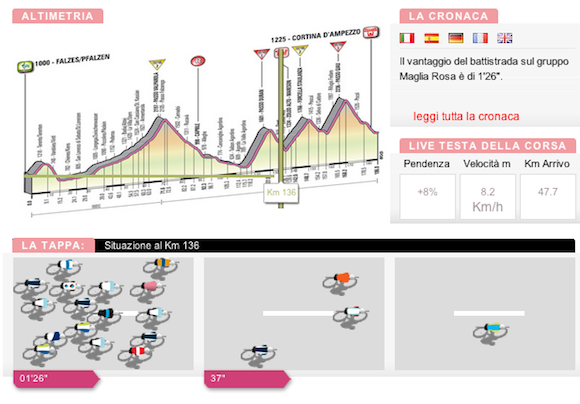
\includegraphics[scale=0.7]{05bericht/images/giro.png}
\end{figure} 

In der Abbildung \ref{fig:giro} ist der Live Abschnitt der offiziellen Webseite zu sehen. Im oberen Teil wird der Standort in der aktuelle Etappe eingeblendet. Unten ist die Situation an der Spitze abgebildet. Die Fahrer sind nach Rückstand gruppiert.
\\

Da jedoch nicht zu erkennen ist, wie die Informationen im Feld erfasst werden, muss die Mitbewerberanalyse an dieser Stelle abgeschlossen werden.